\documentclass[10pt,twocolumn]{article}

\usepackage[margin=0.75in]{geometry}
\usepackage[T1]{fontenc}
\usepackage[utf8]{inputenc}
\usepackage{lmodern}
\usepackage{microtype}
\usepackage{amsmath,amssymb,amsfonts}
\usepackage{booktabs}
\usepackage{graphicx}
\usepackage{subcaption}
\usepackage{float}
\usepackage{multirow}
\usepackage{enumitem}
\usepackage{hyperref}
\usepackage{xcolor}
\usepackage{mathtools}

\hypersetup{
  colorlinks=true,
  linkcolor=blue,
  urlcolor=blue,
  citecolor=blue
}

\title{\bf A Toy-2D Study of Diffusion Posterior Sampling and\\Flow with Interpolant Guidance for Linear Inverse Problems}
\author{Project report extending the original FIG repository with a dedicated toy-2D benchmark}
\date{March 2026}

\begin{document}
\maketitle

\begin{abstract}
This paper presents a complete toy-2D benchmark for comparing Diffusion Posterior Sampling (DPS), plain Flow with Interpolant Guidance (FIG), and FIG+ on linear inverse problems. The study extends the original FIG GitHub repository, which primarily targets image restoration, with a low-dimensional experimental pipeline designed for direct geometric inspection of the posterior. We train compact DDPM priors from scratch on Two-Moons and Eight-Gaussians, define a one-dimensional noisy linear observation model, implement DPS and FIG-family conditional samplers, approximate the reference posterior by importance reweighting, and evaluate the resulting conditional distributions with posterior mean MSE, sliced Wasserstein distance, and measurement consistency. The toy setting makes the solver dynamics visually transparent: one can observe the prior manifold, the observation constraint, and the evolution of samples during denoising. Across the reported experiments, FIG+ is the strongest method on posterior-quality metrics, while plain FIG remains sensitive to the operator structure and tends to underperform on the present mask-like task. The benchmark therefore highlights both the importance of geometry-aware conditioning and the value of toy experiments for interpreting inverse-problem samplers.
\end{abstract}

\section{Introduction}

Diffusion-based priors have become a powerful tool for solving inverse problems, but their behavior is often difficult to interpret in high-dimensional image spaces. Conditional samplers can succeed or fail for several intertwined reasons: the strength of the prior, the choice of solver, the noise schedule, the observation operator, and the geometry of the target posterior. This makes low-dimensional benchmarks especially valuable. In two dimensions, it becomes possible to visualize the entire problem at once: the unconditional prior, the measurement line, the reference conditional distribution, and the trajectories followed by the samplers.

The present work was developed in the context of the original \textit{Flow with Interpolant Guidance} (FIG) repository. That repository provides diffusion- and flow-based algorithms for image restoration tasks such as super-resolution, deblurring, and inpainting. Our goal here is complementary: rather than reproducing the full image pipeline, we construct a self-contained toy-2D environment in which the mechanics of DPS, FIG, and FIG+ can be studied directly.

The resulting benchmark answers three questions:
\begin{enumerate}[leftmargin=1.5em]
    \item Can a compact DDPM prior trained from scratch recover non-Gaussian toy distributions such as Two-Moons and Eight-Gaussians?
    \item How do DPS, plain FIG, and FIG+ behave under a simple one-dimensional linear observation?
    \item Which method best approximates the conditional posterior when the observation leaves one latent coordinate unobserved?
\end{enumerate}

\section{Extension of the Original Repository}

The upstream FIG repository is centered on image inverse problems with strong pretrained priors. It does not provide a dedicated 2D experimental environment. We therefore added the following components:
\begin{itemize}[leftmargin=1.5em]
    \item synthetic data generators for \texttt{two\_moons} and \texttt{eight\_gaussians};
    \item a compact DDPM prior with sinusoidal time embeddings and an MLP denoiser;
    \item a stand-alone training script and checkpointing pipeline for toy-2D priors;
    \item a linear inverse-problem module with Gaussian measurement noise;
    \item modular implementations of DPS, FIG, and FIG+ in the toy setting;
    \item a reference posterior sampler based on importance reweighting of true prior samples;
    \item evaluation scripts exporting CSV summaries, plots, and denoising animations.
\end{itemize}

This extension turns the original repository into a testbed where the conditioning mechanism itself can be examined independently of image-scale architectural complexity.

\section{Problem Setup}

\subsection{Toy Distributions}

We consider two standard non-Gaussian toy datasets:
\begin{itemize}[leftmargin=1.5em]
    \item \textbf{Two-Moons}, a curved bimodal manifold that is useful for studying how conditional sampling behaves on nonlinear supports;
    \item \textbf{Eight-Gaussians}, a strongly multimodal distribution arranged on a ring, well suited to diagnosing mode preservation.
\end{itemize}

\subsection{Diffusion Prior}

For each dataset, we train a DDPM prior from scratch. The forward process is
\begin{equation}
\mathbf{x}_t = \sqrt{\bar{\alpha}_t}\,\mathbf{x}_0 + \sqrt{1-\bar{\alpha}_t}\,\boldsymbol{\epsilon},
\qquad
\boldsymbol{\epsilon} \sim \mathcal{N}(\mathbf{0}, I),
\end{equation}
and the denoiser predicts \(\boldsymbol{\epsilon}_\theta(\mathbf{x}_t,t)\) by minimizing
\begin{equation}
\mathcal{L}_{\mathrm{DDPM}}
=
\mathbb{E}_{\mathbf{x}_0, t, \boldsymbol{\epsilon}}
\left[
\left\|
\boldsymbol{\epsilon} - \boldsymbol{\epsilon}_\theta(\mathbf{x}_t,t)
\right\|_2^2
\right].
\end{equation}

The model is a small MLP with linear layers, SiLU activations, and sinusoidal time embeddings. The reported runs use \(64\) diffusion steps, a cosine schedule, \(8000\) optimization steps, batch size \(1024\), and learning rate \(10^{-3}\).

\begin{figure}[t]
    \centering
    
\includegraphics[width=\columnwidth]{report_assets/two_moons_unconditional_check.png}
    \caption{Sanity check for the learned Two-Moons prior. The diffusion model captures the global geometry of the target distribution sufficiently well to support conditional posterior experiments.}
    \label{fig:prior_check}
\end{figure}

\subsection{Linear Inverse Problem}

We study the noisy linear observation model
\begin{equation}
\mathbf{y} = A\mathbf{x}^\star + \mathbf{n},
\qquad
A = \begin{bmatrix}1 & 0\end{bmatrix},
\qquad
\mathbf{n} \sim \mathcal{N}(\mathbf{0}, \sigma_n^2 I).
\end{equation}

Hence, the first coordinate is observed while the second coordinate remains hidden. Geometrically, conditioning on \(y\) constrains samples to a vertical line, but the posterior along that line remains structured because the prior is non-Gaussian.

\subsection{Reference Posterior and Metrics}

To evaluate the samplers against a meaningful target, we approximate the conditional posterior with importance reweighting. A large pool of exact prior samples \(\{\mathbf{x}^{(i)}\}_{i=1}^N\) is drawn from the true toy distribution, and the weights
\begin{equation}
w_i \propto \exp\left(
-\frac{\|A\mathbf{x}^{(i)} - \mathbf{y}\|_2^2}{2\sigma_n^2}
\right)
\end{equation}
define an empirical approximation of \(p(\mathbf{x}\mid \mathbf{y})\).

We report:
\begin{itemize}[leftmargin=1.5em]
    \item \textbf{Posterior Mean MSE}: error between the mean of generated samples and the mean of the reference posterior;
    \item \textbf{Sliced Wasserstein Distance (SWD)}: discrepancy between the generated and reference conditional distributions;
    \item \textbf{Measurement MSE}: average \(\|A\mathbf{x} - \mathbf{y}\|_2^2\), which quantifies measurement consistency.
\end{itemize}

\section{Conditional Solvers}

\subsection{Diffusion Posterior Sampling}

DPS uses Tweedie's formula to estimate the clean sample
\begin{equation}
\hat{\mathbf{x}}_0
=
\frac{
\mathbf{x}_t - \sqrt{1-\bar{\alpha}_t}\,\boldsymbol{\epsilon}_\theta(\mathbf{x}_t,t)
}{
\sqrt{\bar{\alpha}_t}
}.
\end{equation}
It then evaluates the measurement loss
\begin{equation}
\mathcal{L}_{\mathrm{meas}}^{\mathrm{DPS}}
=
\left\|
\mathbf{y} - A\hat{\mathbf{x}}_0
\right\|_2^2
\end{equation}
and backpropagates that loss to the current noisy state before taking the unconditional DDIM update.

\subsection{Plain FIG}

FIG introduces a measurement interpolant
\begin{equation}
\mathbf{y}_{t-1}
=
\sqrt{\bar{\alpha}_{t-1}}\,\mathbf{y}
+
w\sqrt{1-\bar{\alpha}_{t-1}}\,A\boldsymbol{\epsilon},
\end{equation}
with \(\boldsymbol{\epsilon}\sim\mathcal{N}(\mathbf{0}, I)\), then applies \(K\) gradient steps to the Gaussian negative log-likelihood
\begin{equation}
\mathcal{L}_{\mathrm{meas}}^{\mathrm{FIG}}
=
\frac{1}{2\sigma_n^2}
\left\|
\mathbf{y}_{t-1} - A\mathbf{x}
\right\|_2^2.
\end{equation}

In our implementation, the conditional step is scaled with a noise-dependent factor inspired by the SNR interpretation of the FIG paper:
\begin{equation}
\eta_{t-1}
=
c\,\Delta t\,
\frac{1-\bar{\alpha}_{t-1}}{\bar{\alpha}_{t-1}\,\|A\|_2^2},
\qquad
\Delta t = \frac{1}{T}.
\end{equation}
This provides a practical DDPM-compatible analogue of the theoretical FIG scaling.

\subsection{FIG+ for Mask-Like Operators}

Because the operator \(A=[1,0]\) acts like a coordinate mask, we also study FIG+, which mixes the hidden coordinate with a Tweedie-based estimate. After computing \(\hat{\mathbf{x}}_0\), we perturb it back to the next time level,
\begin{equation}
\tilde{\mathbf{x}}_{t-1}
=
\sqrt{\bar{\alpha}_{t-1}}\,\hat{\mathbf{x}}_0
+
\sqrt{1-\bar{\alpha}_{t-1}}\,\boldsymbol{\epsilon},
\end{equation}
and combine it with the updated state through
\begin{equation}
\mathbf{x}_{t-1}
\leftarrow
P\mathbf{x}_{t-1}
+
(1-m)(I-P)\mathbf{x}_{t-1}
+
m(I-P)\tilde{\mathbf{x}}_{t-1},
\end{equation}
where \(P=\mathrm{diag}(1,0)\) selects the observed coordinate and \(m\in[0,1]\) is a mixing coefficient. Intuitively, this keeps the observed coordinate measurement-consistent while restoring diversity in the hidden component.

\section{Experimental Protocol}

The evaluation is performed on both toy datasets with measurement noise levels
\[
\sigma_n \in \{0.05, 0.5, 1.0\}.
\]
For each dataset and each noise level, we use:
\begin{itemize}[leftmargin=1.5em]
    \item \(6\) test observations;
    \item \(128\) conditional samples per solver and per observation;
    \item \(128\) reference posterior samples;
    \item a \(20{,}000\)-sample importance pool for posterior approximation.
\end{itemize}

For plain FIG and FIG+, we ablate
\[
K \in \{1,3,5\},
\qquad
w \in \{0.0, 0.5\}.
\]
In all result tables, the reported FIG and FIG+ entries correspond to the best \((K,w)\) configuration according to posterior mean MSE.

\section{Results}

\subsection{Quantitative Results on Two-Moons}

\begin{table*}[t]
\centering
\small
\caption{Two-Moons results. Lower is better for all metrics.}
\begin{tabular}{lcccccc}
\toprule
\(\sigma_n\) & Solver & Best \((K,w)\) & Posterior Mean MSE & SWD & Measurement MSE \\
\midrule
0.05 & DPS & -- & 0.083 & 0.362 & \(1.24\times 10^{-2}\) \\
0.05 & FIG & (5, 0.5) & 0.580 & 1.040 & \(1.02\times 10^{-1}\) \\
0.05 & FIG+ & (5, 0.5) & 0.004 & 0.140 & \(7.28\times 10^{-3}\) \\
\midrule
0.50 & DPS & -- & 0.127 & 0.465 & \(8.51\times 10^{-3}\) \\
0.50 & FIG & (5, 0.0) & 0.069 & 0.324 & \(1.27\times 10^{-1}\) \\
0.50 & FIG+ & (3, 0.5) & 0.018 & 0.285 & \(3.54\times 10^{-2}\) \\
\midrule
1.00 & DPS & -- & 0.196 & 0.674 & \(2.00\times 10^{-2}\) \\
1.00 & FIG & (5, 0.5) & 0.025 & 0.472 & \(5.30\times 10^{-1}\) \\
1.00 & FIG+ & (5, 0.0) & 0.051 & 0.541 & \(2.01\times 10^{-1}\) \\
\bottomrule
\end{tabular}
\label{tab:two_moons}
\end{table*}

\begin{figure*}[t]
    \centering
    
\includegraphics[width=\textwidth]{report_assets/two_moons_paper_metric_trends.png}
    \caption{Two-Moons quantitative trends. FIG+ is strongest on posterior-quality metrics across the tested noise levels, whereas plain FIG shows a pronounced trade-off between posterior quality and measurement fidelity.}
    \label{fig:two_moons_trends}
\end{figure*}

Two-Moons is especially informative because the posterior often remains bimodal along the observation line. DPS already captures that geometry reasonably well, but FIG+ is consistently stronger in posterior mean MSE and SWD. Plain FIG performs well only in part of the grid and remains less reliable overall.

\subsection{Quantitative Results on Eight-Gaussians}

\begin{table*}[t]
\centering
\small
\caption{Eight-Gaussians results. Lower is better for all metrics.}
\begin{tabular}{lcccccc}
\toprule
\(\sigma_n\) & Solver & Best \((K,w)\) & Posterior Mean MSE & SWD & Measurement MSE \\
\midrule
0.05 & DPS & -- & 0.335 & 0.947 & 1.228 \\
0.05 & FIG & (5, 0.0) & 3.070 & 1.904 & 0.285 \\
0.05 & FIG+ & (5, 0.0) & 0.004 & 0.337 & 0.021 \\
\midrule
0.50 & DPS & -- & 0.273 & 0.819 & 1.307 \\
0.50 & FIG & (5, 0.0) & 3.200 & 1.955 & 0.937 \\
0.50 & FIG+ & (5, 0.5) & 0.019 & 0.362 & 0.153 \\
\midrule
1.00 & DPS & -- & 0.266 & 0.798 & 1.311 \\
1.00 & FIG & (5, 0.5) & 2.136 & 1.691 & 1.580 \\
1.00 & FIG+ & (3, 0.0) & 0.028 & 0.429 & 0.813 \\
\bottomrule
\end{tabular}
\label{tab:eight_gaussians}
\end{table*}

\begin{figure*}[t]
    \centering
    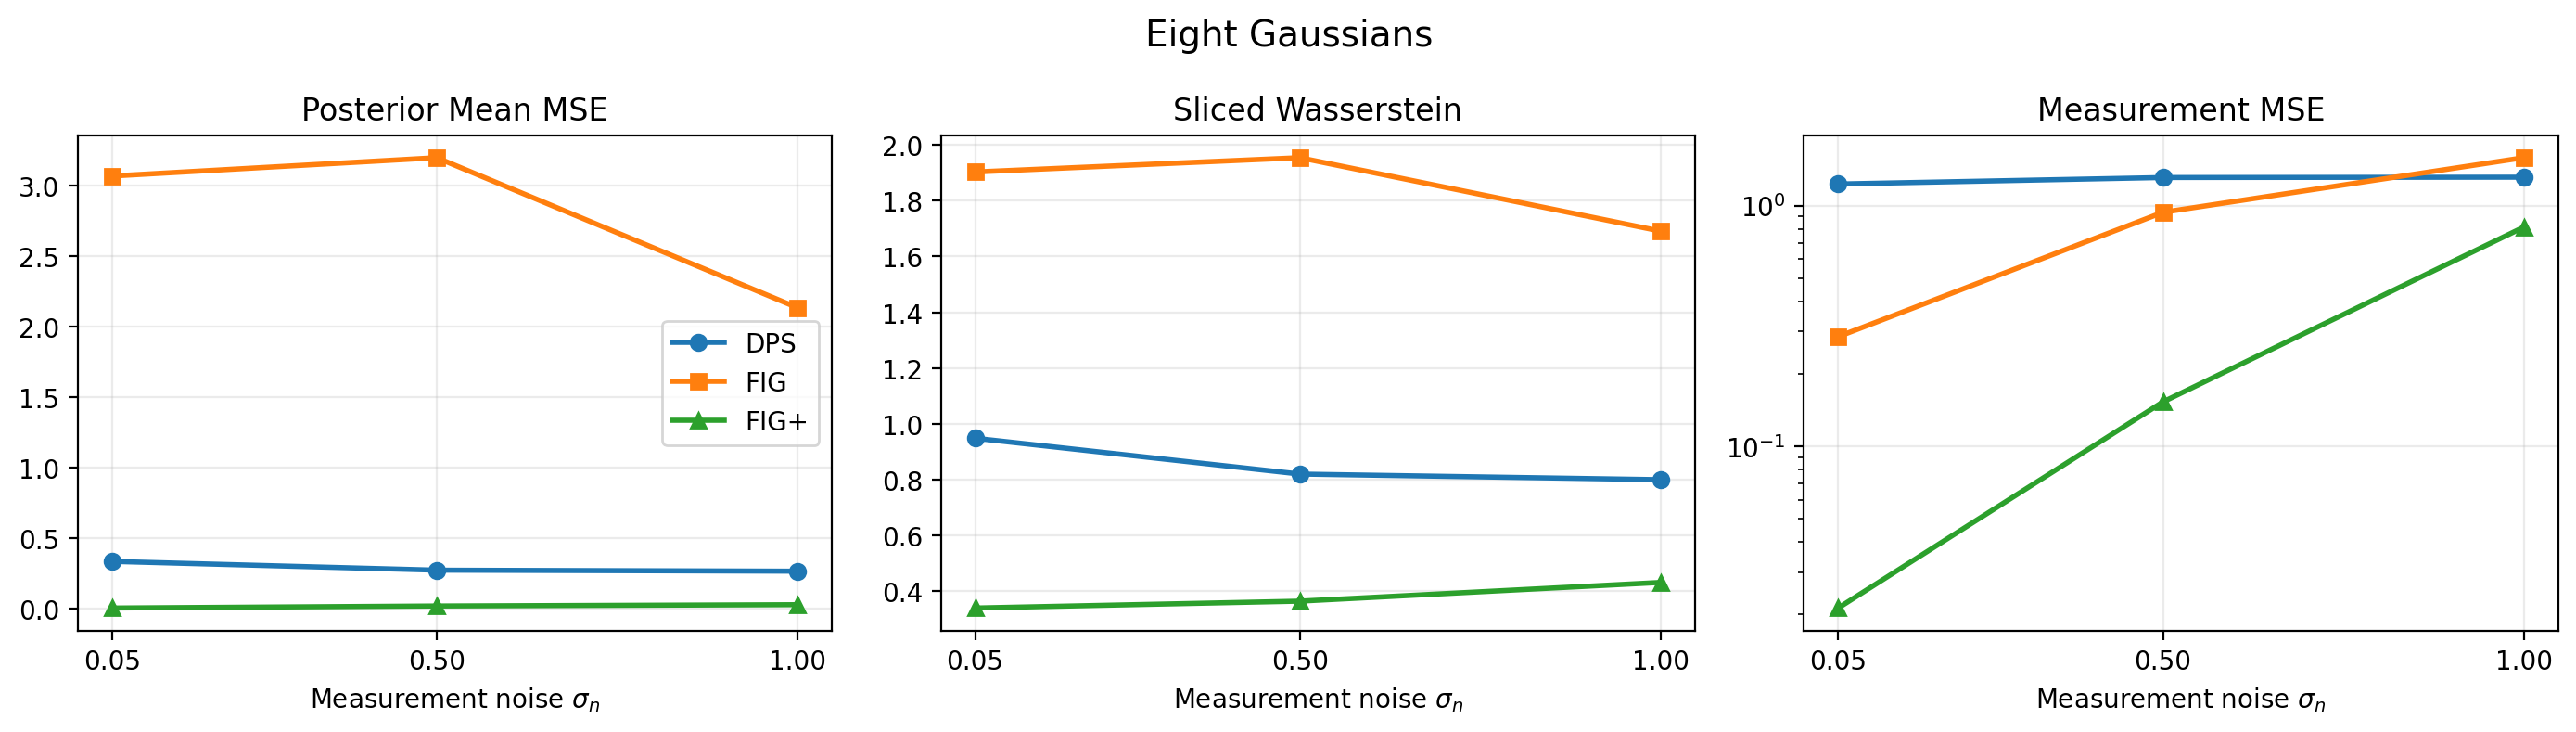
\includegraphics[width=\textwidth]{report_assets/eight_gaussians_paper_metric_trends.png}
    \caption{Eight-Gaussians quantitative trends. The multimodal geometry makes the ranking particularly clear: FIG+ is substantially closer to the reference posterior than either DPS or plain FIG.}
    \label{fig:eight_trends}
\end{figure*}

Eight-Gaussians makes the mode-preservation issue even clearer. Because several clusters remain plausible under the observed first coordinate, the solver must preserve multimodality rather than collapse toward a narrow conditional column. In this regime, FIG+ is clearly the strongest sampler of the three.

\subsection{Qualitative Comparisons}

\begin{figure*}[t]
    \centering
    \begin{subfigure}{0.49\textwidth}
        \centering
        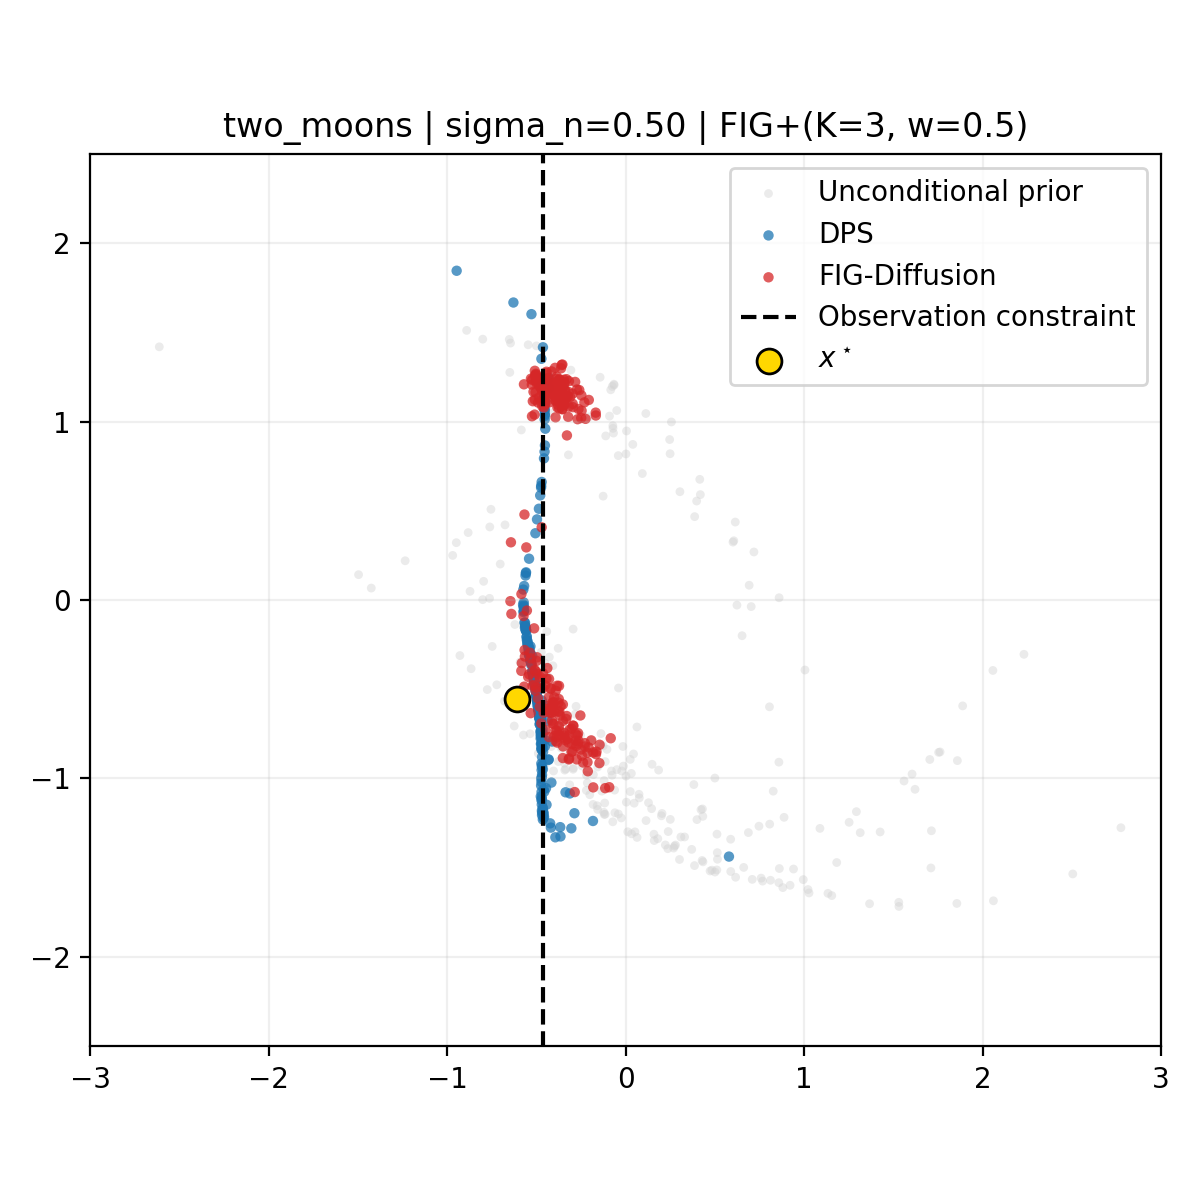
\includegraphics[width=\textwidth]{report_assets/qualitative/two_moons_sigma_0.50_dps_vs_fig_plus.png}
        \caption{Two-Moons, \(\sigma_n=0.5\).}
    \end{subfigure}
    \hfill
    \begin{subfigure}{0.49\textwidth}
        \centering
        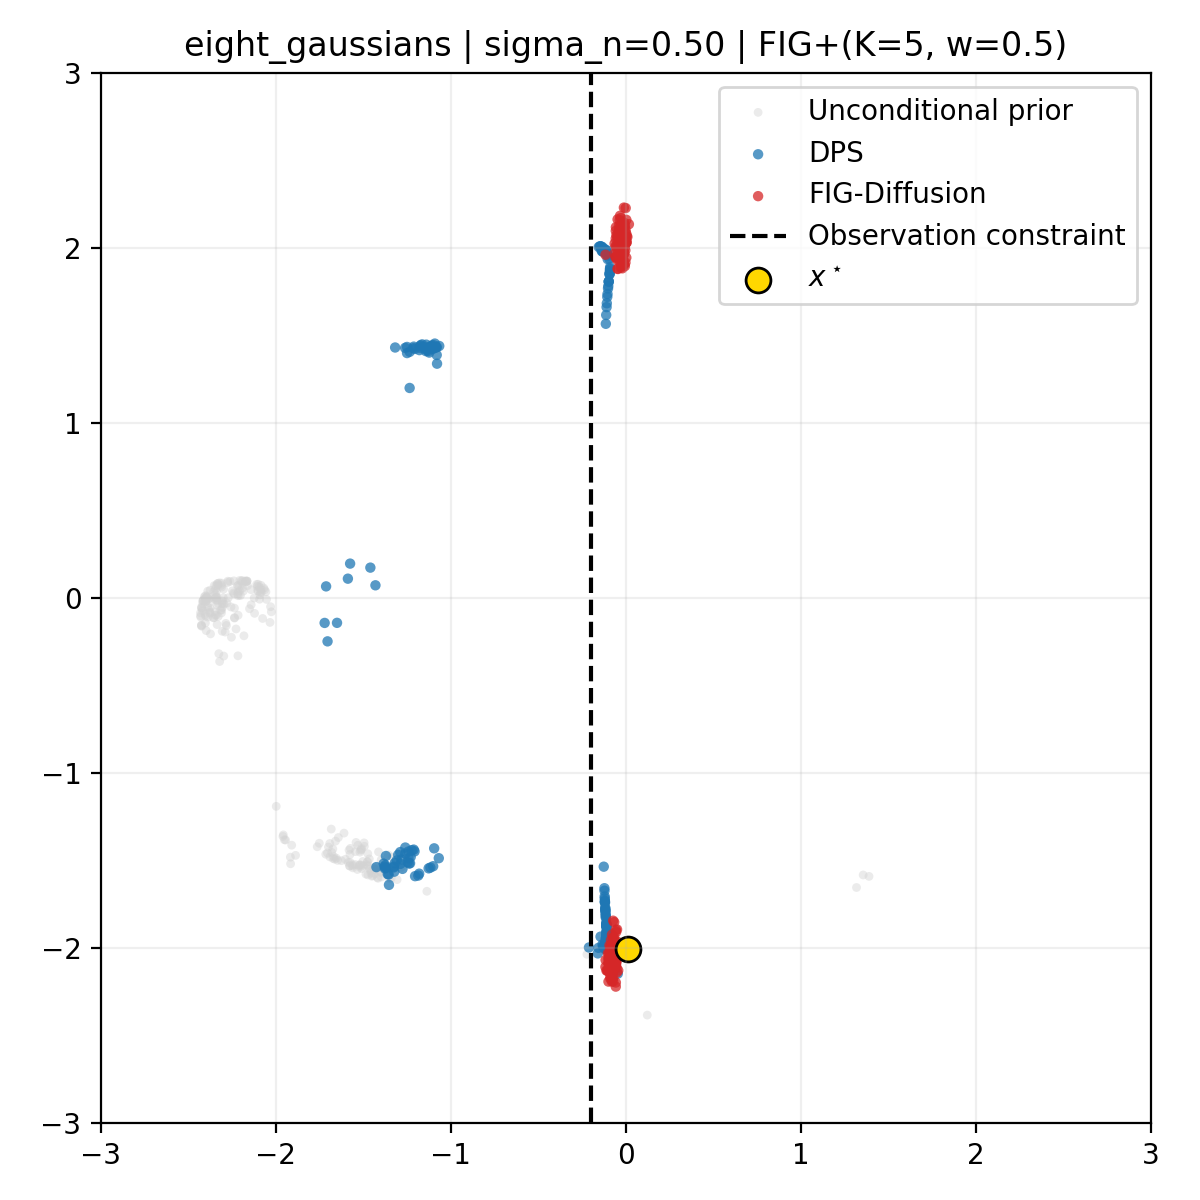
\includegraphics[width=\textwidth]{report_assets/qualitative/eight_gaussians_sigma_0.50_dps_vs_fig_plus.png}
        \caption{Eight-Gaussians, \(\sigma_n=0.5\).}
    \end{subfigure}
    \caption{Representative conditional sample clouds for DPS and FIG+. The gray background shows unconditional prior samples, the dashed line is the observation constraint, and the colored clouds are conditional samples. FIG+ typically remains closer to the conditional structure of the prior while still enforcing the measurement.}
    \label{fig:qualitative}
\end{figure*}

The qualitative plots confirm the quantitative picture. On both datasets, FIG+ maintains a conditional cloud that is visibly more compatible with the reference geometry of the prior under the measurement constraint.

\subsection{Denoising Dynamics}

Static sample clouds only show the endpoint of the solver. To inspect the mechanism itself, we also generated denoising animations from a shared noisy initialization. The most informative case is Two-Moons with a fixed ambiguous measurement \(y=0\) and low measurement noise \(\sigma_n=0.05\). In this setting, the target posterior is bimodal along the vertical line \(x=0\).

\begin{figure*}[t]
    \centering
    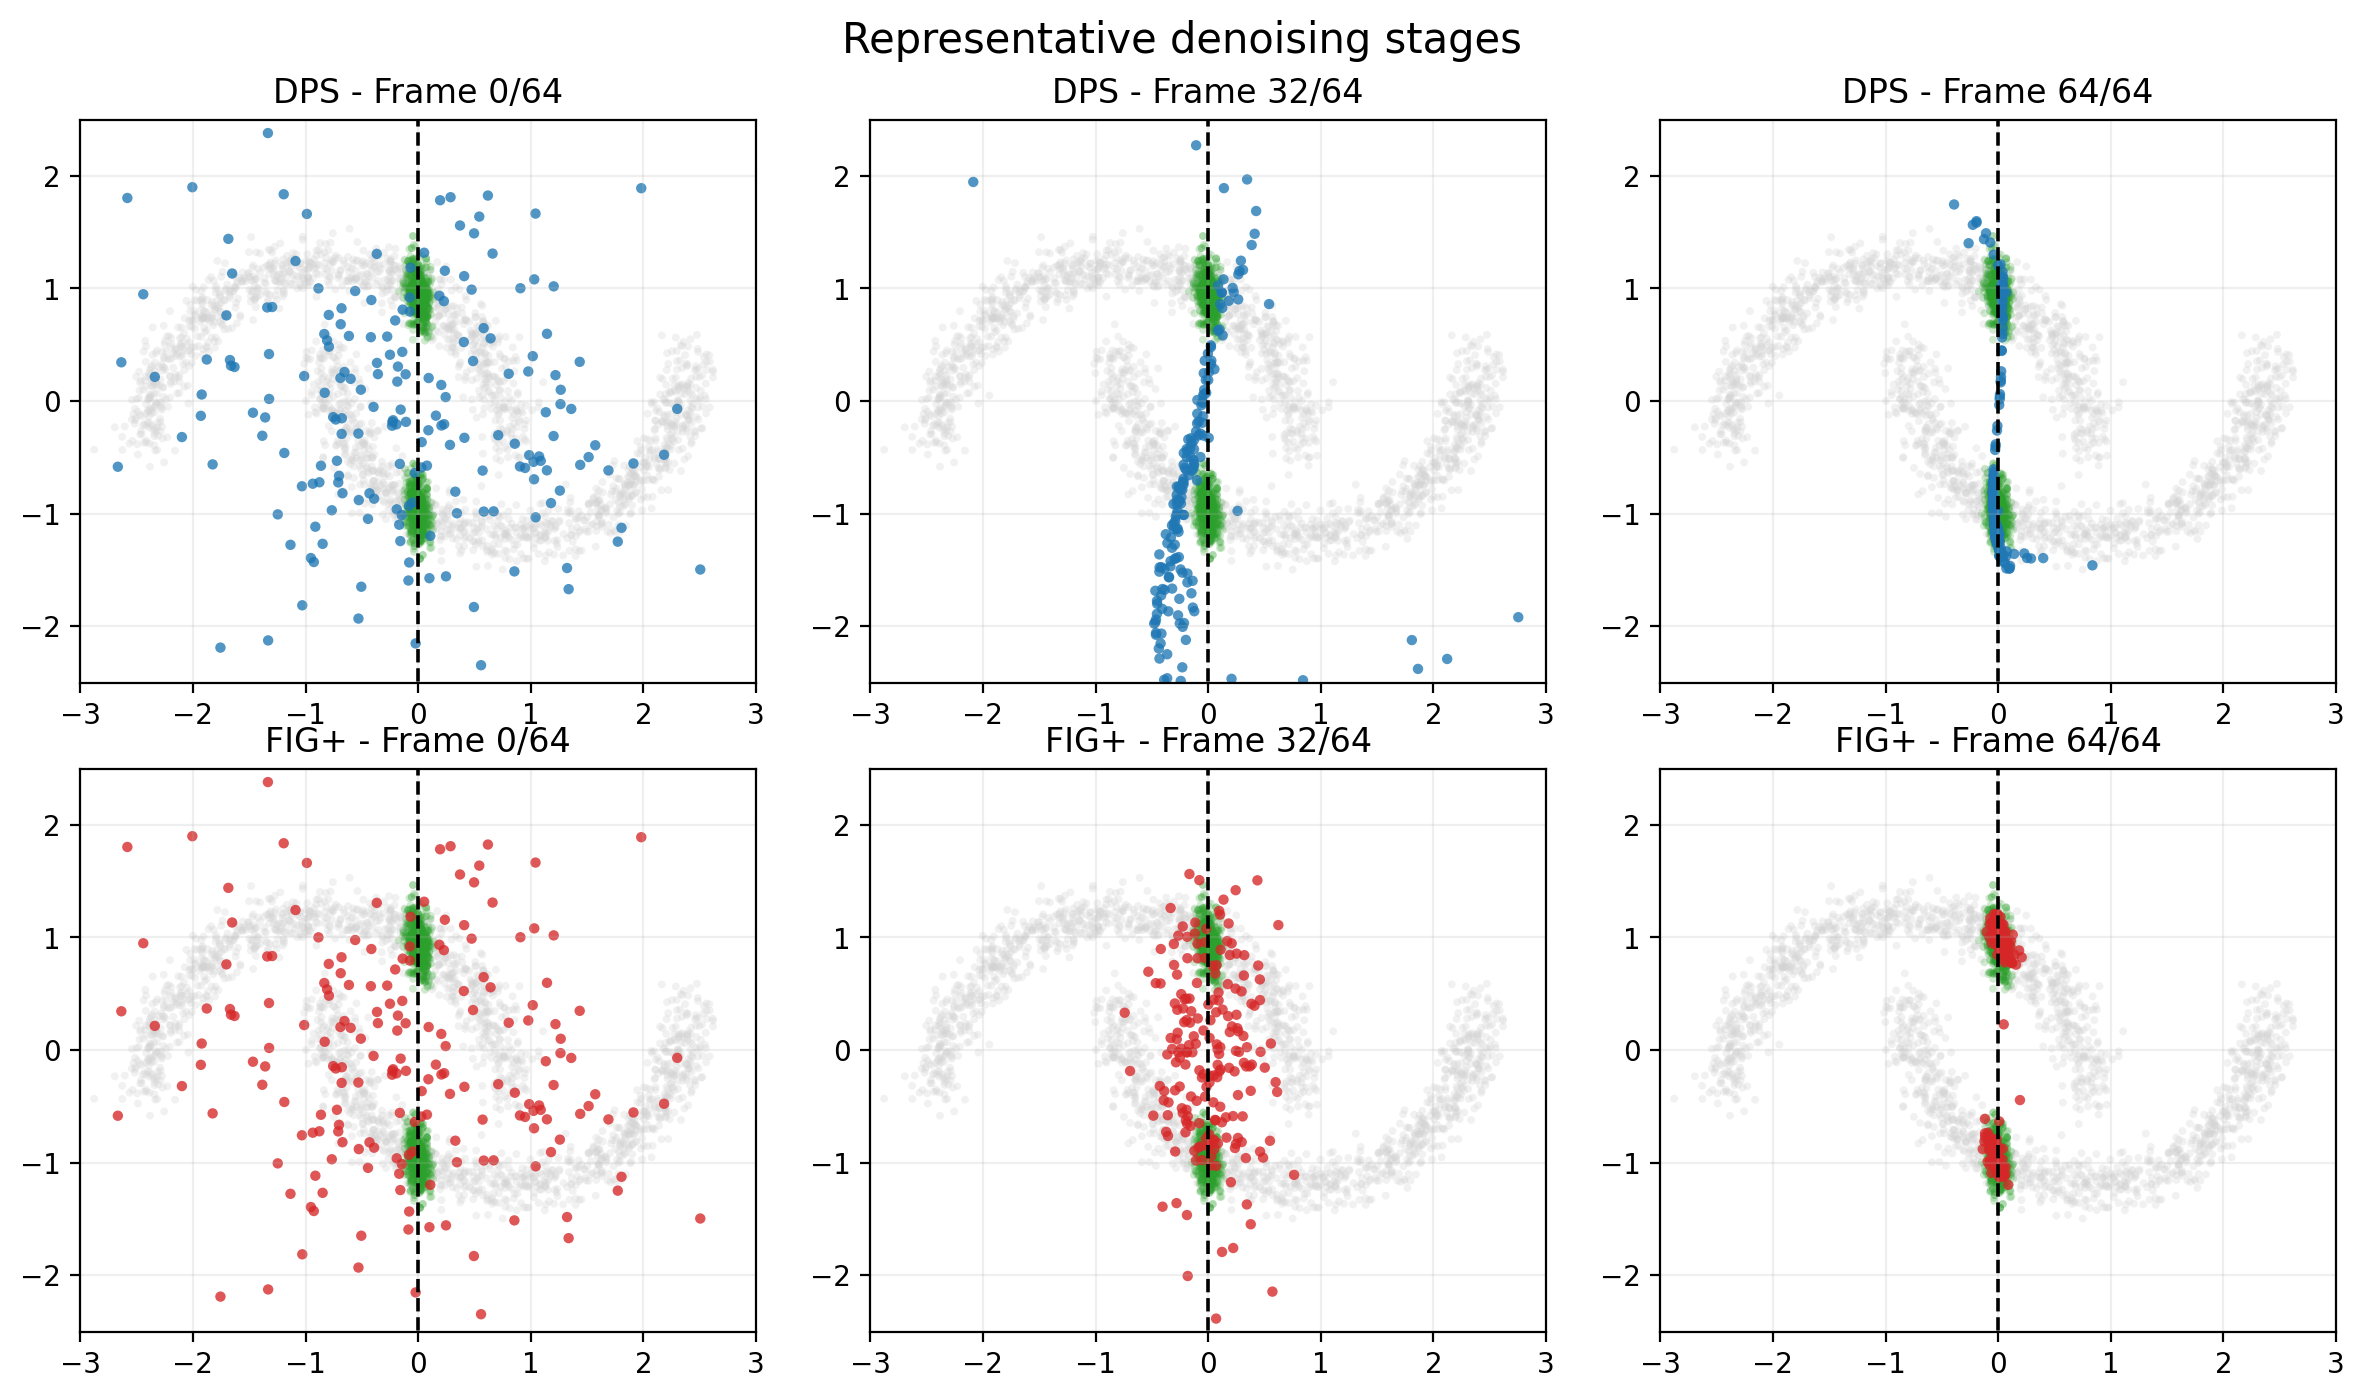
\includegraphics[width=\textwidth]{animations/two_moons_sigma_0.05_dps_vs_fig_plus_strip.png}
    \caption{Representative frames from the DPS-vs-FIG+ denoising trajectory. Gray denotes the unconditional prior support and green denotes the reference posterior obtained by importance reweighting. Both samplers start from the same noisy cloud, but FIG+ reaches the two posterior modes more sharply.}
    \label{fig:dynamics}
\end{figure*}

The full animation is available alongside the paper at
\begin{center}
\texttt{animations/two\_moons\_sigma\_0.05\_dps\_vs\_fig\_plus.gif}.
\end{center}
This dynamic view is particularly useful because it shows not only where the samplers end, but how they reshape the cloud as the noise level decreases.

\section{Discussion}

Several conclusions emerge from the benchmark.

\paragraph{1. The toy-2D setting is highly informative.}
The experiment makes the posterior geometry directly visible, which is difficult to achieve in image space. It becomes immediately clear when a solver respects multimodality and when it collapses too strongly toward the observation manifold.

\paragraph{2. FIG+ is the strongest method for the present operator.}
Because the observation hides one coordinate entirely, the task has a mask-like structure. In that regime, the Tweedie-based mixing of FIG+ provides a decisive advantage over both DPS and plain FIG.

\paragraph{3. Plain FIG is more sensitive to operator structure.}
The base interpolant-guided update is often effective at enforcing the measurement, but it does not preserve the hidden-coordinate geometry as well as FIG+ in the present experiments. This is most visible on Eight-Gaussians, where several modes remain plausible after conditioning.

\paragraph{4. Posterior fidelity and measurement consistency are distinct objectives.}
Low measurement MSE does not necessarily imply good posterior reconstruction. A sampler can be perfectly aligned with the observation while still missing the correct conditional spread. The joint use of posterior mean MSE, SWD, and measurement MSE is therefore essential.

\section{Limitations and Future Work}

The current paper focuses on a deliberately minimal setting. Several extensions would be natural:
\begin{itemize}[leftmargin=1.5em]
    \item larger evaluation sweeps with more test observations and more reference samples;
    \item additional linear operators, including rotated projections and full-rank noisy maps;
    \item nonlinear observation models;
    \item stronger diffusion priors or score models;
    \item a direct bridge from the toy benchmark back to the image-scale operators of the original FIG repository.
\end{itemize}

These directions would help separate which phenomena are generic properties of the solver and which are specific to the present mask-like inverse problem.

\section{Conclusion}

This work transforms the original FIG repository into a complete toy-2D benchmark for inverse problems. The benchmark is compact enough to be interpretable and rich enough to reveal meaningful differences between conditional samplers. In the reported experiments, DPS is a strong baseline, plain FIG is competitive only in part of the grid, and FIG+ is the most effective method overall on posterior-quality metrics. More broadly, the study shows why toy benchmarks are valuable: they expose the geometry of conditional generation directly and make algorithmic behavior observable rather than merely measurable.

\section*{Practical Note}

No LaTeX engine was available on the current machine at generation time, so this source is provided ready to compile, together with all figures and animation assets referenced above.

\end{document}
